% ============================================================
%  PRÉSENTATION BEAMER — État d'avancement du mémoire
%  Auteur  : NDZESSA AVELE BRUNO LANDRY
%  Titre   : Plateforme gouvernementale pour la cartographie
%             et la mise en relation des besoins des entreprises
%  ENSPM — Université de Maroua | 2025/2026
% ============================================================

\documentclass[aspectratio=169, 10pt]{beamer}

% ------------------------------------------------------------
%  THÈME DE BASE
% ------------------------------------------------------------
\usetheme{Madrid}
\usecolortheme{default}
\usepackage{tikz}
\usetikzlibrary{positioning}
\usetikzlibrary{shapes.geometric}
\usepackage{graphicx}
\usepackage{float}
\usepackage{subcaption} % Requis pour les sous-figures
% Exemple de définitions de couleurs si nécessaire
\definecolor{primary}{RGB}{0, 51, 102}
\definecolor{secondary}{RGB}{204, 102, 0}
\definecolor{darkgray}{RGB}{80, 80, 80}
% ------------------------------------------------------------
%  ENCODAGE & LANGUE
% ------------------------------------------------------------
\usepackage[utf8]{inputenc}
\usepackage[T1]{fontenc}
\usepackage[french]{babel}
\usepackage{csquotes}

% ------------------------------------------------------------
%  POLICES
% ------------------------------------------------------------
\usepackage{lmodern}
\usepackage{microtype}

% ------------------------------------------------------------
%  MATHS
% ------------------------------------------------------------
\usepackage{amsmath, amssymb}
\usepackage{bm}

% ------------------------------------------------------------
%  GRAPHIQUES & TABLEAUX
% ------------------------------------------------------------
\usepackage{graphicx}
\usepackage{booktabs}
\usepackage{tabularx}
\usepackage{multirow}
\usepackage{colortbl}
\usepackage{tikz}
\usetikzlibrary{shapes, arrows.meta, positioning, calc}

% ------------------------------------------------------------
%  COULEURS — reprises du mémoire
% ------------------------------------------------------------
\definecolor{primary}{RGB}{0, 51, 102}
\definecolor{secondary}{RGB}{0, 102, 153}
\definecolor{accent}{RGB}{200, 50, 50}
\definecolor{lightgray}{RGB}{245, 245, 245}
\definecolor{darkgray}{RGB}{80, 80, 80}
\definecolor{successgreen}{RGB}{34, 139, 34}

% ------------------------------------------------------------
%  PERSONNALISATION DU THÈME BEAMER
% ------------------------------------------------------------
\setbeamercolor{palette primary}{bg=primary, fg=white}
\setbeamercolor{palette secondary}{bg=secondary, fg=white}
\setbeamercolor{palette tertiary}{bg=primary!80, fg=white}
\setbeamercolor{palette quaternary}{bg=primary, fg=white}
\setbeamercolor{structure}{fg=primary}
\setbeamercolor{section in toc}{fg=primary}
\setbeamercolor{frametitle}{bg=primary, fg=white}
\setbeamercolor{title}{bg=primary, fg=white}
\setbeamercolor{block title}{bg=primary, fg=white}
\setbeamercolor{block body}{bg=primary!8, fg=black}
\setbeamercolor{block title alerted}{bg=accent, fg=white}
\setbeamercolor{block body alerted}{bg=accent!8, fg=black}
\setbeamercolor{block title example}{bg=successgreen!80, fg=white}
\setbeamercolor{block body example}{bg=successgreen!8, fg=black}
\setbeamercolor{itemize item}{fg=primary}
\setbeamercolor{itemize subitem}{fg=secondary}
\setbeamercolor{enumerate item}{fg=primary}

\setbeamerfont{frametitle}{series=\bfseries}
\setbeamerfont{title}{series=\bfseries, size=\large}
\setbeamerfont{block title}{series=\bfseries}

% Navigation simplifiée
\setbeamertemplate{navigation symbols}{}
\setbeamertemplate{footline}{
    \leavevmode
    \hbox{%
        \begin{beamercolorbox}[wd=.33\paperwidth, ht=2.25ex, dp=1ex, center]{palette primary}
            \usebeamerfont{author in head/foot}\insertshortauthor
        \end{beamercolorbox}%
        \begin{beamercolorbox}[wd=.34\paperwidth, ht=2.25ex, dp=1ex, center]{palette secondary}
            \usebeamerfont{title in head/foot}\insertshorttitle
        \end{beamercolorbox}%
        \begin{beamercolorbox}[wd=.33\paperwidth, ht=2.25ex, dp=1ex, center]{palette primary}
            \usebeamerfont{date in head/foot}
            \insertframenumber{} / \inserttotalframenumber
        \end{beamercolorbox}%
    }
    \vskip0pt%
}

% Séparateur de section
\AtBeginSection[]{
    \begin{frame}
        \vfill
        \centering
        \begin{beamercolorbox}[sep=12pt, center, rounded=true, shadow=true]{palette primary}
            \usebeamerfont{title}
            \insertsectionhead\par
        \end{beamercolorbox}
        \vfill
    \end{frame}
}

% ------------------------------------------------------------
%  MÉTADONNÉES
% ------------------------------------------------------------
\title[Cartographie des besoins entreprises]{%
    Conception et développement d'une plateforme gouvernementale\\
    pour la cartographie des besoins et la mise en relation\\
    des entreprises locales}

\subtitle{Présentation de l'état d'avancement}

\author[NDZESSA AVELE Bruno Landry]{%
    \textbf{NDZESSA AVELE BRUNO LANDRY}
    \small Matricule : 21D0180EP}

\institute[ENSPM — Maroua]{%
    École Nationale Supérieure Polytechnique de Maroua\\
    Département d'Informatique et Télécommunications\\[4pt]
    \small Directeur : Pr Mohamadou Alidou\\
    Encadreur académique: Pr Kaladzavi\\
    Encadreur professionnel: M. Abdoulaziz Junmbe
    }

\date{Année académique 2025 / 2026}

% ============================================================
%  DOCUMENT
% ============================================================
\begin{document}

% -----------------------------------------------------------
%  DIAPO 1 — PAGE DE TITRE
% -----------------------------------------------------------
\begin{frame}[plain]
    \titlepage
\end{frame}

% -----------------------------------------------------------
%  DIAPO 2 — PLAN
% -----------------------------------------------------------
\begin{frame}{Plan de la présentation}
    \tableofcontents[hideallsubsections]
\end{frame}

% ============================================================
\section{Contexte et problématique}
% ============================================================

% -----------------------------------------------------------
%  DIAPO 3 — Cadre institutionnel
% -----------------------------------------------------------
\begin{frame}{Cadre institutionnel}
    \begin{columns}[T]
        \begin{column}{0.58\textwidth}
            \begin{block}{Structure d'accueil}
                \begin{itemize}
                    \item \textbf{MINEPAT} — Ministère de l'Économie,
                          de la Planification et de l'Aménagement du Territoire
                    \item \textbf{DAPE} — Division des Analyses
                          et des Politiques Économiques
                    \item Rattachée à la \textbf{DGEPIP}
                \end{itemize}
            \end{block}
            \vspace{6pt}
            \begin{alertblock}{Mission de la DAPE}
                \begin{itemize}
                	\item Analyse économique: Analyser les évolutions de la conjoncture économique nationale et internationale;
                	\item Suivi des politiques: Evaluer l'impact des politiques économiques, sectorielles et des réformes structurelles sur le developpement du pays;
                	 
                \end{itemize}
            \end{alertblock}
        \end{column}
        \begin{column}{0.38\textwidth}
            \centering
            \begin{tikzpicture}[
                node distance=0.8cm,
                box/.style={rectangle, draw=primary, fill=primary!10,
                    text width=3cm, align=center, rounded corners=3pt,
                    minimum height=0.7cm, font=\scriptsize},
                line/.style={->, thick, color=primary}
                ]
                \node[box, fill=primary, text=white] (min) {Ministre};
                \node[box, below=of min] (sg) {Secrétariat Général};
                \node[box, below=of sg] (dg) {DGEPIP};
                \node[box, below=of dg, fill=secondary!30,
                    draw=secondary, font=\scriptsize\bfseries] (dape)
                    {DAPE\\{\tiny lieu de stage}};
                \draw[line] (min) -- (sg);
                \draw[line] (sg) -- (dg);
                \draw[line] (dg) -- (dape);
            \end{tikzpicture}
        \end{column}
    \end{columns}
\end{frame}

% -----------------------------------------------------------
%  DIAPO 4 — Problématique
% -----------------------------------------------------------
\begin{frame}{Contexte \& Problématique}
    \begin{columns}[T]
        \begin{column}{0.45\textwidth}
            \begin{alertblock}{Context}
                \begin{itemize}
                    \item Dans de nombreux pays, le secteur privé jout un role déterminant dans la production des biens et services ainsi que la création de la valeur ajoutée;
                    \item Au travers des trois piliers de la SND30, le Cameroun se fixe comme objectif le developpement du secteur privé moteur de la croissance économique;
                    \item Des réformes ont donc été engagées, des indicateurs de croissances définis;
                    \item L'évaluation mi-parcourt de l'atteinte des indicateurs de croissance de la SND30 fait état d'une économie Camerounaise résiliente mais bien loin des idéaux fixés.
                \end{itemize}
            \end{alertblock}
        \end{column}
        \begin{column}{0.51\textwidth}
            \begin{exampleblock}{Problèmatique}
                \begin{enumerate}
                    \item Le secteur privé est incontournable pour une croissance économique d'un pays et au Cameroun ce secteur rencontre d'énorme difficulté;
           
                    \item Permettre au secteur privé de contribuer à la croissance économique consisterait pour l'administration centrale d'aider les entreprises privées à se défaire des besoins qui les retardent;
                    \item Bien d'initiatives ont été engagées dans l'optique sus-cité avec des résultats peut concluant;
                    \item Une enquete en vue du rescencement des besoins des entreprises est lancée par le MINEPAT en 2025. 
                \end{enumerate}
            \end{exampleblock}
        \end{column}
    \end{columns}
    \vspace{8pt}
    
\end{frame}
\begin{block}{Question centrale}
	\centering
	\textit{Comment exploiter les données issues de cette enquete pour dynamiser le secteur privé moteur de la croissance économique?}
\end{block}
% ============================================================
\section{Sources de données et résultats de l'analyse descriptive}
% ============================================================

% -----------------------------------------------------------
%  DIAPO 5 — Source des données
% -----------------------------------------------------------
\begin{frame}{Source des données : enquête MINEPAT 2025}
    \begin{columns}[T]
        \begin{column}{0.38\textwidth}
            \begin{block}{Dispositif de collecte}
                \begin{itemize}
                    \item Enquête sur les besoins des entreprises;
                    \item Outil de collecte: Plateforme numérique pour la centralisation des données;
                    \item Couverture~: Toutes les régions du Cameroun
                    \item Les données ont été stockées dans une base de données MySQL contenant deux tables (identifications et besoins)
                \end{itemize}
            \end{block}
        \end{column}
        \begin{column}{0.58\textwidth}
            \begin{block}{Variables descriptives et les besoins retenues }
                \begin{enumerate}
                    \item Dans nos travaux la description des entreprises a porté sur les variables:Raison sociale, region, taille, statut, secteur d'activité,date de debut des activités 
                    \item Les besoins des entreprises retenues sont:
                    besoins\_intrants, besoins\_financement, besoins\_emballages, besoins\_transport, besoins\_appui\_entreprises, besoins\_equipements, besoins\_innovation\_recherche;
                    \item Une jonction entre les deux tables (identifications, besoins) a été réalisée;
                    \item Une ligne représente une entreprise et la présence d'un besoin ou pas se traduit par les variables catégorielles Oui ou Non.
                \end{enumerate}
            \end{block}
        \end{column}
    \end{columns}
\end{frame}

% -----------------------------------------------------------
%  DIAPO 6 — Résultats analyse bivariée (tableau chi2)
% -----------------------------------------------------------
\begin{frame}{Résultat de l'analyse descriptive}
    \footnotesize
    \begin{figure}[H]
    	\centering
    	% --- Première ligne d'images ---
    	\begin{subfigure}[b]{0.32\textwidth}
    		\centering
    		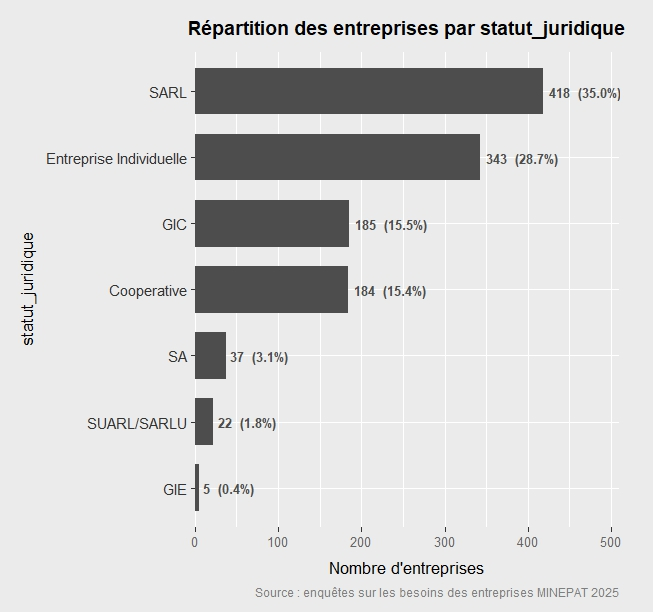
\includegraphics[width=\textwidth]{statut.jpeg}
    		\caption{Répartition des entreprises par statut juridique}
    		\label{fig:sous_fig_a}
    	\end{subfigure}
    	\hfill % Espace horizontal entre les images
    	\begin{subfigure}[b]{0.32\textwidth}
    		\centering
    		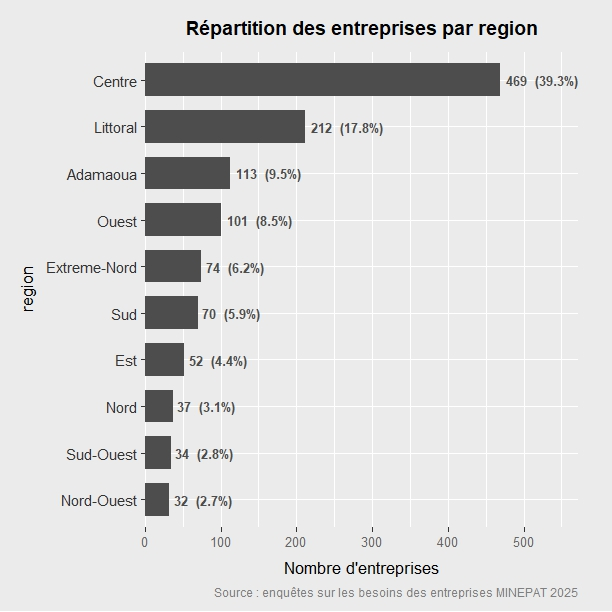
\includegraphics[width=\textwidth]{repartition_region.jpeg}
    		\caption{Répartition des entreprises par région}
    		\label{fig:sous_fig_b}
    	\end{subfigure}
    	\hfill
    	\begin{subfigure}[b]{0.32\textwidth}
    		\centering
    		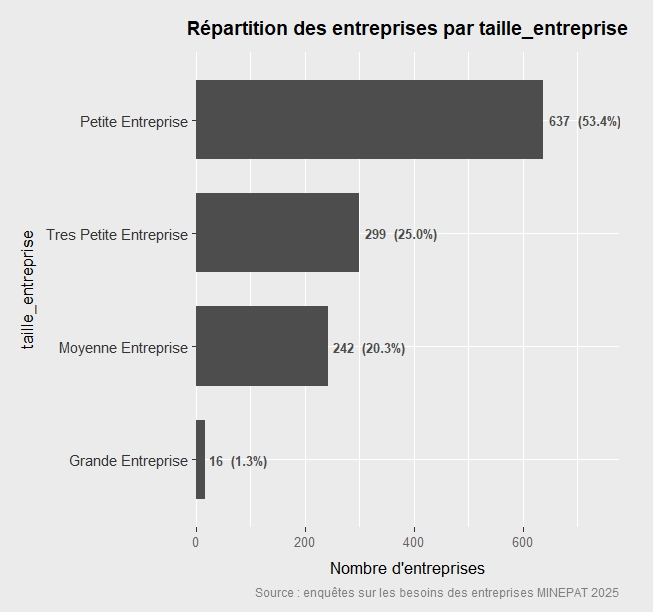
\includegraphics[width=\textwidth]{repartition_taille.jpeg}
    		\caption{Répartition des entreprises par taille}
    		\label{fig:sous_fig_c}
    	\end{subfigure}
    	
    	\vspace{0.5cm} % Espace vertical entre les deux lignes d'images
    	
    	% --- Deuxième ligne d'images ---
    	
    	% --- Légende globale ---
    	
    \end{figure}

\end{frame}
\begin{figure}[H]
	\begin{subfigure}[b]{0.42\textwidth}
		\centering
		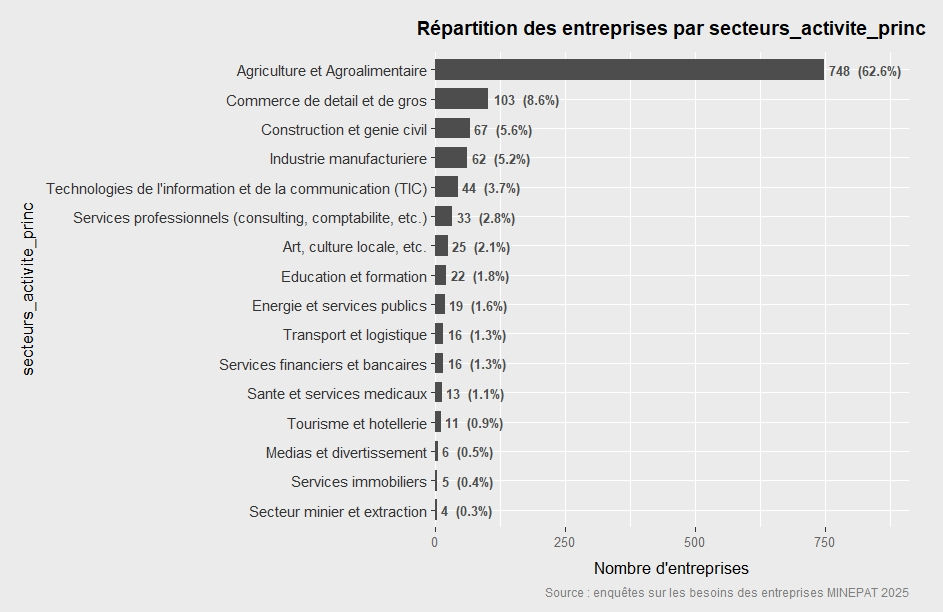
\includegraphics[width=\textwidth]{repartition_activite.jpeg}
		\caption{Répartition des entreprises par secteur d'activité}
		\label{fig:sous_fig_d}
	\end{subfigure}
	\hfill
	\begin{subfigure}[b]{0.52\textwidth}
		\centering
		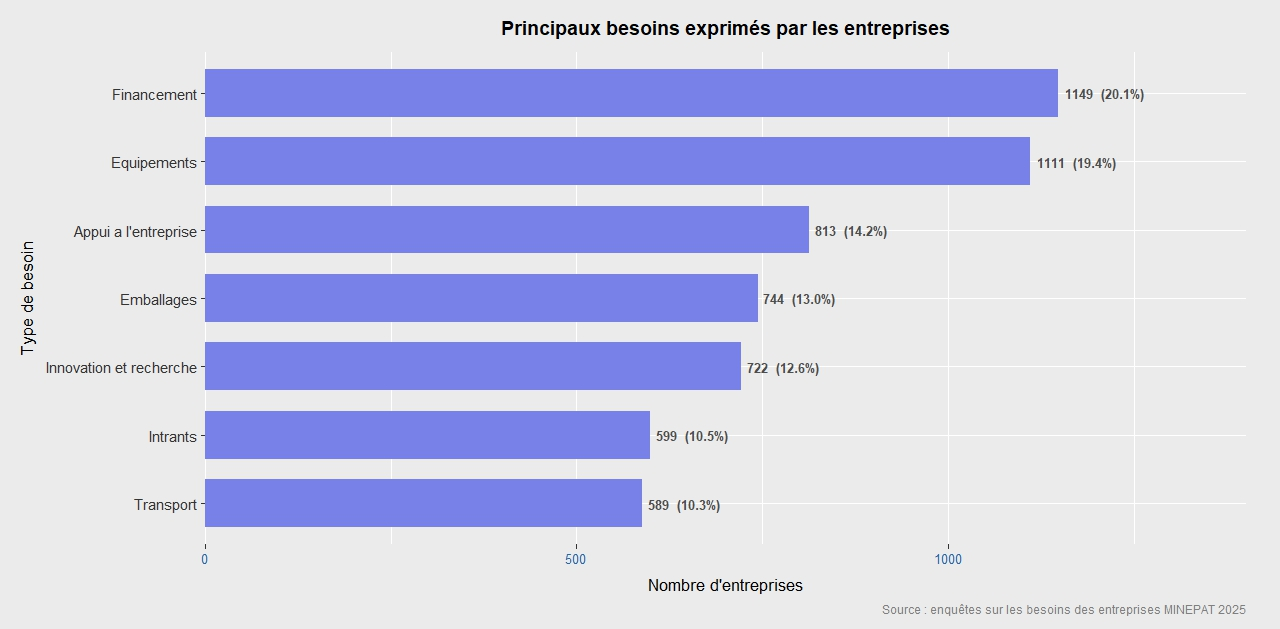
\includegraphics[width=\textwidth]{repartition_besoins.jpeg}
		\caption{Répartition des besoins des entreprises}
		\label{fig:sous_fig_e}
	\end{subfigure}
	\caption{Répartition des entreprises selon leurs variables descriptives et leurs besoins (Total\_entreprise: 1194)}
	\label{fig:besoins_secteur_global}
\end{figure}
\vspace{6pt}
\begin{alertblock}{Résultat clé}
	On observe qu'il y'a très peu de grande entreprise (1,3\%), plus de la moitié des entreprises sont des Petites entreprises(53,4\%). C'est la région du Centre qui dénombre le plus grand nombre d'entreprises(39,3\%) suivi par la région du Littoral(17,8\%) ce qui pourrait susciter des interrogations du fait que la capitale économique soit dans le Littoral. 62,6\% Des entreprises évoluent dans le secteur de l' Agriculture et Agroalimentaire et les besoins les plus réccurents sont le financement(20,1\%), Equipements(19,4\%). Les autres besoins bien qu'ayant des pourcentages d'apparition moindre sont assez bien représentés. 
\end{alertblock}

% --- Diapositive 1 : Tableau Synthétique ---
\begin{frame}{Synthèse de l'Analyse Bivariée (Test $\chi^2$ et $V$ de Cramér)}
	\begin{center}
		\scriptsize % Taille de police adaptée au tableau
		\renewcommand{\arraystretch}{1.2}
		\begin{tabular}{l|ccccc}
			\toprule
			\textbf{Besoins exprimés} & \textbf{Statut} & \textbf{Région} & \textbf{Ancien.} & \textbf{Secteur} & \textbf{Taille} \\
			\midrule
			Besoin en intrants & \cellcolor{green!15}0,11 & \cellcolor{green!15}0,16 & Non & \cellcolor{green!15}0,29 & Non \\
			
			\rowcolor{gray!5}
			Besoin en financement & Non & Non & Non & \cellcolor{green!15}0,17 & Non \\
			
			Besoin en emballages & \cellcolor{green!15}0,19 & \cellcolor{green!15}0,13 & Non & \cellcolor{blue!15}\textbf{0,51} & Non \\
			
			\rowcolor{gray!5}
			Besoin en transport & \cellcolor{green!15}0,21 & \cellcolor{green!15}0,16 & Non & \cellcolor{green!15}0,35 & Non \\
			
			Appui aux entreprises & \cellcolor{green!15}0,15 & \cellcolor{green!15}0,14 & \cellcolor{green!10}0,10 & Non & \cellcolor{green!10}0,11 \\
			
			\rowcolor{gray!5}
			Besoin en équipements & \cellcolor{green!15}0,23 & \cellcolor{green!15}0,15 & \cellcolor{green!10}0,11 & \cellcolor{blue!15}\textbf{0,45} & Non \\
			
			Innovation \& Recherche & \cellcolor{green!15}0,26 & \cellcolor{green!15}0,14 & \cellcolor{green!10}0,13 & \cellcolor{green!15}0,37 & Non \\
			\midrule
			\textbf{Significativité} & \textbf{6 / 7} & \textbf{6 / 7} & \textbf{3 / 7} & \textbf{6 / 7} & \textbf{1 / 7} \\
			\bottomrule
		\end{tabular}
	\end{center}
	\vfill
	\begin{itemize}
		\item \tiny \textbf{Légende :} Les valeurs indiquent le coefficient $V$ de Cramér pour les tests significatifs ($p < 0,05$). 
		\item \tiny \color{blue!80}\textbf{Bleu} : Association très forte ($V > 0,40$). \color{black} | \color{gray}\textbf{Non} : Test non significatif.
	\end{itemize}
\end{frame}

% --- Diapositive 2 : Enseignements Clés ---
\begin{frame}{Principaux Enseignements de l'Analyse}
	\begin{itemize}
		\item \textbf{Le Secteur d'Activité : Déterminant n°1}
		\begin{itemize}
			\item Le secteur d'activité influence grandement les besoins matériels : Emballages ($V=0,51$) et Équipements ($V=0,45$).
		\end{itemize}
		\vfill
		\item \textbf{L'Universalité du Besoin en Financement}
		\begin{itemize}
			\item \alert{Exception statistique} : Ne dépend ni de la taille, ni de la région, ni de l'ancienneté. 
			\item C'est une contrainte structurelle transversale à tout le tissu économique.
		\end{itemize}
		\vfill
		\item \textbf{Logique de Cycle de Vie}
		\begin{itemize}
			\item \textbf{Jeunes/Petites structures} : Priorité à l'amorçage (équipements et appui institutionnel).
			\item \textbf{Entreprises matures (20 ans+)} : Virage vers la compétitivité (Innovation \& Recherche).
		\end{itemize}
		\vfill
		\item \textbf{Disparités Régionales}
		\begin{itemize}
			\item Besoins en \textbf{transport} et \textbf{intrants} marqués dans les zones enclavées (Nord-Ouest, Est, Adamaoua), reflétant les défis infrastructurels.
		\end{itemize}
	\end{itemize}
\end{frame}
% ============================================================
\section{Résultat de l' analyse multidimentionnelle }
% ============================================================

% -----------------------------------------------------------
%  DIAPO 7 — Pipeline méthodologique
% -----------------------------------------------------------
\begin{frame}{Pipeline d'analyse}
	\centering
	\begin{tikzpicture}[
		node distance=0.6cm and 1.2cm,
		box/.style={rectangle, draw=primary, fill=primary!12,
			text width=2.5cm, align=center, rounded corners=4pt,
			minimum height=1.1cm, font=\small\bfseries},
		arrow/.style={->, very thick, color=primary},
		txtlabel/.style={font=\scriptsize\itshape, color=darkgray, align=center} % Corrigé : nom unique + align=center
		]
		\node[box] (acm) {ACM};
		\node[box, right=of acm] (cah) {CAH};
		\node[box, right=of cah] (afd) {AFD};
		\node[box, right=of afd, fill=secondary!20, draw=secondary] (plat)
		{Plateforme\\de mise en\\relation};
		
		\draw[arrow] (acm) -- (cah);
		\draw[arrow] (cah) -- (afd);
		\draw[arrow] (afd) -- (plat);
		
		\node[txtlabel, below=0.15cm of acm]
		{Réduction\\de dimension};
		\node[txtlabel, below=0.15cm of cah]
		{Partition en\\3 classes};
		\node[txtlabel, below=0.15cm of afd]
		{Validation \& \\prédiction};
		\node[txtlabel, below=0.15cm of plat]
		{Recommandation\\ciblée};
	\end{tikzpicture}
	
	\vspace{10pt}
	\begin{columns}[T]
		\begin{column}{0.3\textwidth}
			\begin{block}{\hfill ACM\hfill} % Corrigé : centrage propre
				\centering\scriptsize
				Variables qualitatives\\
				$\downarrow$\\
				Axes factoriels\\
				(DVS de $\mathbf{S}$)
			\end{block}
		\end{column}
		\begin{column}{0.3\textwidth}
			\begin{block}{\hfill CAH\hfill} % Corrigé : centrage propre
				\centering\scriptsize
				Coordonnées factorielles\\
				$\downarrow$\\
				Critère de Ward\\
				3 classes
			\end{block}
		\end{column}
		\begin{column}{0.3\textwidth}
			\begin{block}{\hfill AFD\hfill} % Corrigé : centrage propre
				\centering\scriptsize
				Classes connues\\
				$\downarrow$\\
				Critère de Fisher\\
				Règle de Bayes
			\end{block}
		\end{column}
	\end{columns}
\end{frame}
% -----------------------------------------------------------
%  DIAPO 8 — ACM : principe et équations
% -----------------------------------------------------------
\begin{frame}{ACM — Analyse des Correspondances Multiples}
    \begin{columns}[T]
        \begin{column}{0.48\textwidth}
            \begin{block}{Principe}
                \begin{itemize}
                    \item Tableau disjonctif complet
                          $\mathbf{Z} \in \{0,1\}^{n \times K}$
                    \item Matrice des profils~:
                          $\mathbf{P} = \tfrac{1}{nQ}\mathbf{Z}$
                    \item Matrice à décomposer~:
                \end{itemize}
                \vspace{4pt}
                \[
                    \mathbf{S} = \mathbf{D}_r^{-1/2}
                    \!\left(\mathbf{P} - \mathbf{r}\mathbf{c}^{\top}\right)
                    \!\mathbf{D}_c^{-1/2}
                \]
            \end{block}
        \end{column}
        \begin{column}{0.48\textwidth}
            \begin{block}{DVS et projections}
                Décomposition~: $\mathbf{S} = \mathbf{U}\boldsymbol{\Sigma}\mathbf{V}^{\top}$
                \vspace{4pt}
                \begin{itemize}
                    \item Valeurs propres~:
                          $\lambda_s = \sigma_s^2$
                    \item Coordonnées individus~:
                          \[
                              \mathbf{F} =
                              \mathbf{D}_r^{-1/2}\mathbf{U}\boldsymbol{\Sigma}
                          \]
                    \item Coordonnées modalités~:
                          \[
                              \mathbf{G} =
                              \mathbf{D}_c^{-1/2}\mathbf{V}\boldsymbol{\Sigma}
                          \]
                \end{itemize}
            \end{block}
        \end{column}
    \end{columns}
    \vspace{6pt}
    \begin{exampleblock}{Propriété barycentrique}
        Les individus sont représentés au barycentre de leurs modalités~;
        les modalités au barycentre des individus qui les possèdent.
    \end{exampleblock}
\end{frame}
% --- DIAPOSITIVE 1 : Objectif & Choix des axes ---
\begin{frame}{ACM : Objectif et Choix des Axes (Éboulis des VP)}
	\begin{columns}[c]
		\begin{column}{0.55\textwidth}
			\begin{figure}
				\centering
				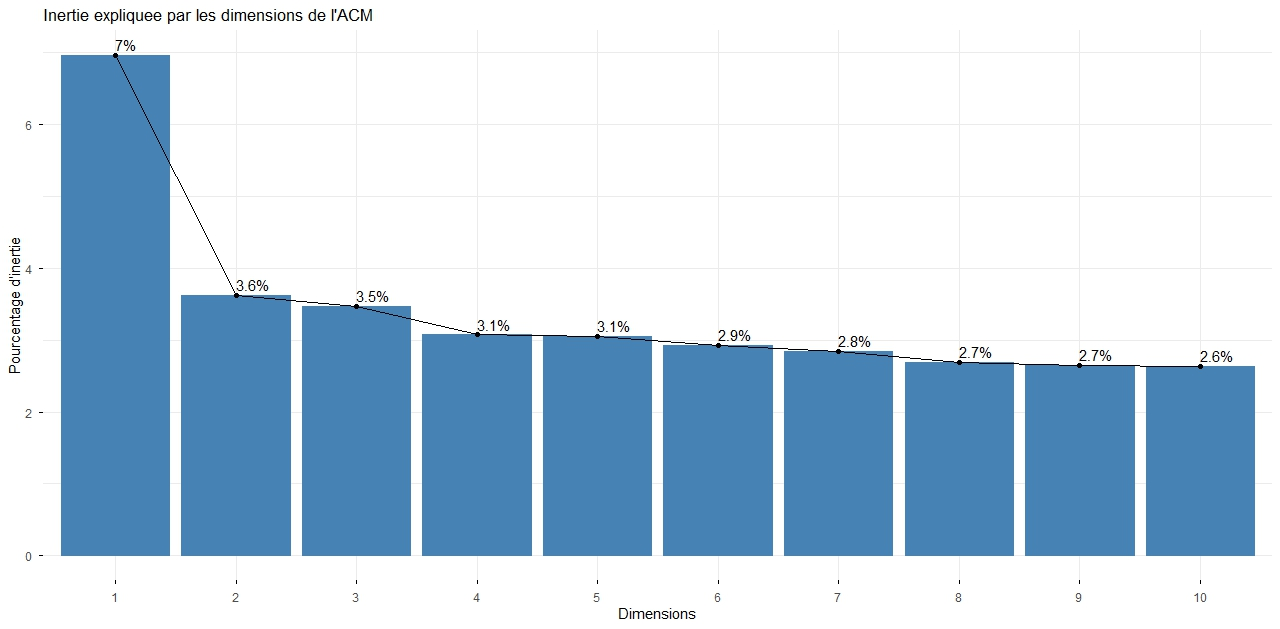
\includegraphics[width=\textwidth]{contributionValeursPropres.jpeg}
				\caption{\label{fig:acm_vp}Éboulis des valeurs propres}
			\end{figure}
		\end{column}
		
		\begin{column}{0.42\textwidth}
			\textbf{Objectif de l'ACM :}
			\begin{itemize}
				\item Synthétiser le nuage d'entreprises à partir des variables qualitatives (\texttt{FactoMineR}).
			\end{itemize}
			\vfill
			\textbf{Critère du « coude » :}
			\begin{itemize}
				\item Pente raide (information forte) puis aplatissement (bruit de fond).
				\item \alert{\textbf{Sélection : 5 premiers axes}} factoriels retenus pour l'analyse.
			\end{itemize}
		\end{column}
	\end{columns}
\end{frame}


% --- DIAPOSITIVE 2 : Premier plan factoriel ---
\begin{frame}{Projection des Modalités (Axes 1 \& 2)}
	\begin{center}
		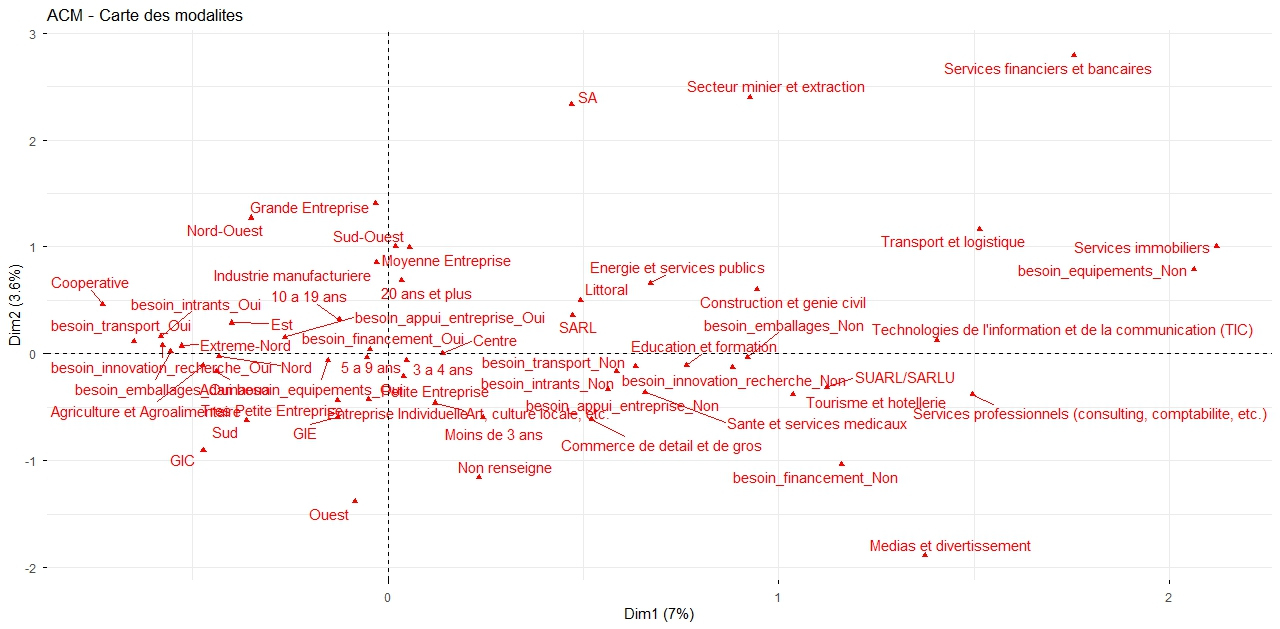
\includegraphics[width=0.7\textwidth]{projectionDesCategories.jpeg}
	\end{center}
	\begin{block}{Interprétation des Axes}
		\begin{itemize}
			\item \textbf{Axe 1 (Horizontal) :} Oppose les entreprises du tertiaire au secteur primaire (via la nature des besoins et secteurs).
			\item \textbf{Axe 2 (Vertical) :} Discrimine les structures selon leur \textbf{statut juridique} et leur \textbf{taille}.
			\item \alert{\textbf{Fait marquant :}} Le \textit{besoin en financement} est situé quasi au centre $\rightarrow$ \textbf{besoin transversal} à toutes les entreprises.
		\end{itemize}
	\end{block}
\end{frame}


% --- DIAPOSITIVE 3 : Contributions Axe 1 ---
\begin{frame}{Contributions à l'Axe 1 : Besoins Opérationnels (7\% d'inertie)}
	\begin{columns}[c]
		\begin{column}{0.5\textwidth}
			\begin{figure}
				\centering
				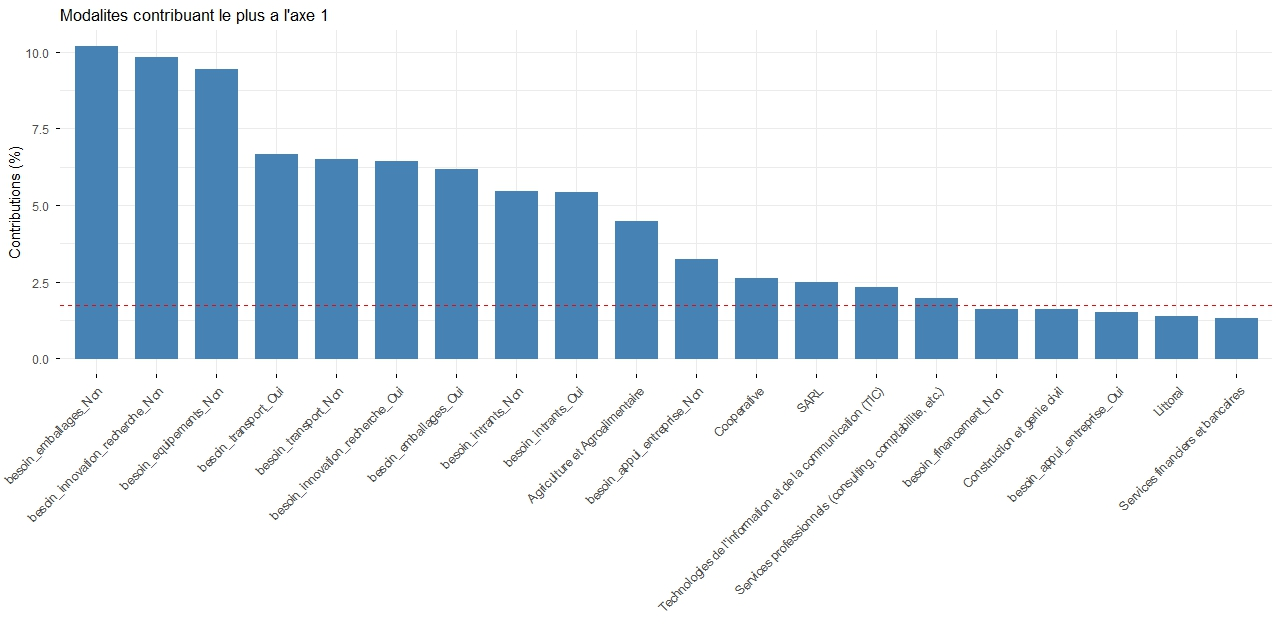
\includegraphics[width=\textwidth]{contributionCategoriesAlAxe1.jpeg}
				\caption{Contributions à l'Axe 1}
			\end{figure}
		\end{column}
		
		\begin{column}{0.48\textwidth}
			\textbf{Un axe dicté par les besoins matériels et techniques :}
			\begin{itemize}
				\item \textbf{Top 3 des modalités (>10\% chacune) :} 
				\begin{itemize}
					\item \texttt{besoin\_emballages\_Non}
					\item \texttt{besoin\_innovation\_Non}
					\item \texttt{besoin\_equipements\_Non}
				\end{itemize}
				\item \textbf{Effet miroir (5\% à 7\%) :} Présence vs absence des besoins logistiques (\texttt{transport}, \texttt{emballages}, \texttt{innovation}).
			\end{itemize}
			\begin{exampleblock}{Synthèse Axe 1}
				Dichotomie nette entre la présence et l'absence de besoins matériels et technologiques.
			\end{exampleblock}
		\end{column}
	\end{columns}
\end{frame}


% --- DIAPOSITIVE 4 : Contributions Axe 2 ---
\begin{frame}{Contributions à l'Axe 2 : Structure Institutionnelle (3.6\% d'inertie)}
	\begin{columns}[c]
		\begin{column}{0.5\textwidth}
			\begin{figure}
				\centering
				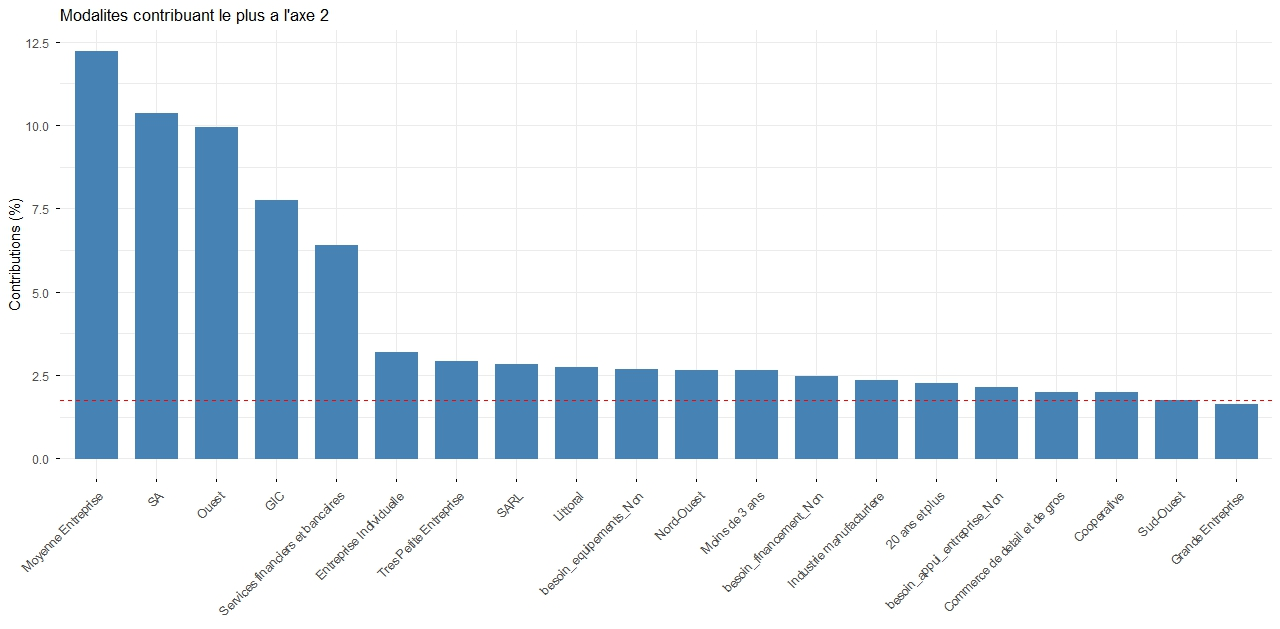
\includegraphics[width=\textwidth]{contributionCategorieALAxe2.jpeg}
				\caption{Contributions à l'Axe 2}
			\end{figure}
		\end{column}
		
		\begin{column}{0.48\textwidth}
			\textbf{Rupture totale : Axe purement statutaire et géographique}
			\begin{itemize}
				\item \textbf{5 piliers majeurs (au-dessus du seuil) :}
				\begin{enumerate}
					\item \textbf{Moyenne Entreprise} ($\sim$12\%)
					\item Forme juridique \textbf{SA} ($\sim$10.5\%)
					\item Région de l'\textbf{Ouest} ($\sim$10\%)
					\item Statut de \textbf{GIC} ($\sim$7.5\%)
					\item Secteur \textbf{Finances/Banques} ($\sim$6.5\%)
				\end{enumerate}
				\item L'âge et les besoins opérationnels n'ont aucune influence ici.
			\end{itemize}
			\begin{exampleblock}{Synthèse Axe 2}
				Capte spécifiquement le niveau de formalisation légale et la structuration des entités.
			\end{exampleblock}
		\end{column}
	\end{columns}
\end{frame}
% -----------------------------------------------------------
%  DIAPO 9 — CAH : critère de Ward
% -----------------------------------------------------------
\begin{frame}{CAH — Classification Ascendante Hiérarchique}
    \begin{columns}[T]
        \begin{column}{0.52\textwidth}
            \begin{block}{Algorithme de Ward}
                Fusion itérative des paires minimisant la
                perte d'inertie inter-classes~:
                \[
                    \Delta(C_a, C_b)
                    = \frac{n_a \cdot n_b}{n_a + n_b}
                      \left\|\bar{x}_a - \bar{x}_b\right\|^2
                \]
                Distance entre individus (espace ACM)~:
                \[
                    d(\omega_i, \omega_j)
                    = \sqrt{\sum_{s=1}^{q}(F_{is} - F_{js})^2}
                \]
            \end{block}
        \end{column}
        \begin{column}{0.44\textwidth}
            \begin{exampleblock}{Choix de 3 classes}
                \begin{itemize}
                    \item Coupure du dendrogramme
                          guidée par le saut d'inertie
                    \item Lisibilité opérationnelle
                          pour la plateforme
                    \item Trois profils distincts~:
                          \begin{itemize}
                              \item[\textbullet] Profil productif
                              \item[\textbullet] Profil financier
                              \item[\textbullet] Profil innovation
                          \end{itemize}
                \end{itemize}
            \end{exampleblock}
        \end{column}
    \end{columns}
\end{frame}
% --- DIAPOSITIVE 1 : Méthodologie & Dendrogramme ---
\begin{frame}{CAH : Méthodologie et Choix de la Partition}
	\begin{columns}[c]
		\begin{column}{0.52\textwidth}
			\begin{figure}
				\centering
				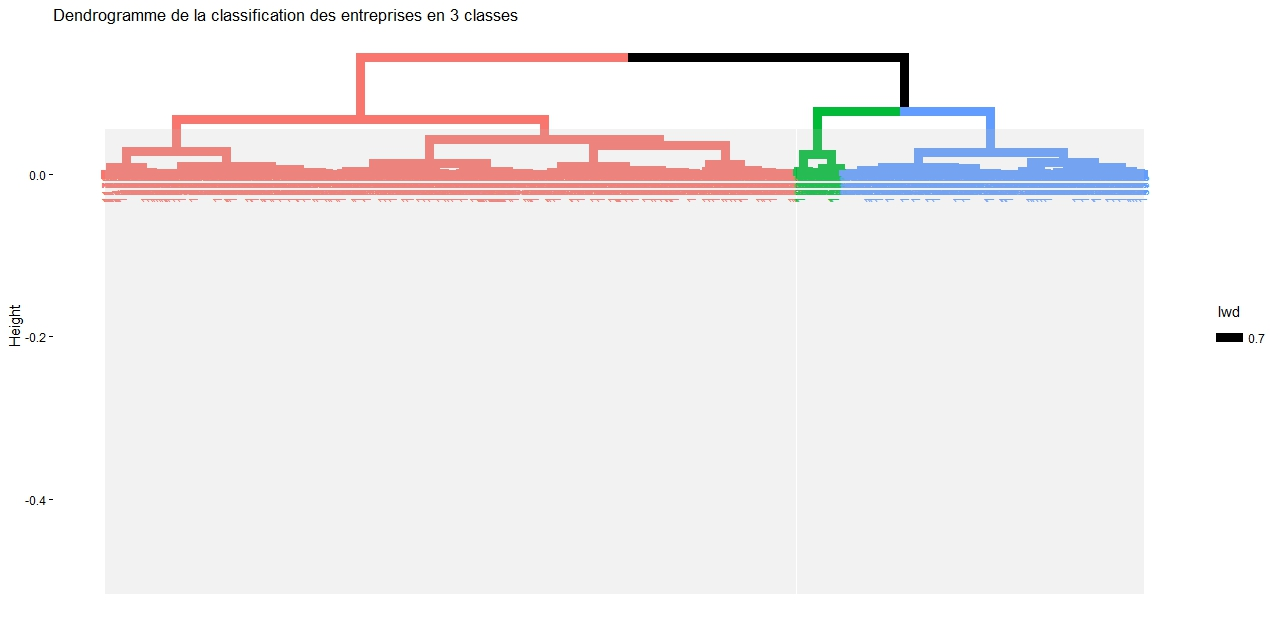
\includegraphics[width=\textwidth]{dendrogramme.jpeg}
				\caption{Dendrogramme (Méthode de Ward)}
			\end{figure}
		\end{column}
		
		\begin{column}{0.45\textwidth}
			\textbf{Approche méthodologique :}
			\begin{itemize}
				\item CAH basée sur les coordonnées factorielles de l'ACM.
				\item Critère de Ward (minimisation de la perte d'inertie intra-classe).
			\end{itemize}
			\vfill
			\textbf{Le choix des 3 classes :}
			\begin{itemize}
				\item Valeur fixée
			\end{itemize}
		\end{column}
	\end{columns}
\end{frame}


% --- DIAPOSITIVE 2 : Projection sur le plan factoriel ---
\begin{frame}{Projection de la Partition sur le Premier Plan Factoriel}
	\begin{center}
		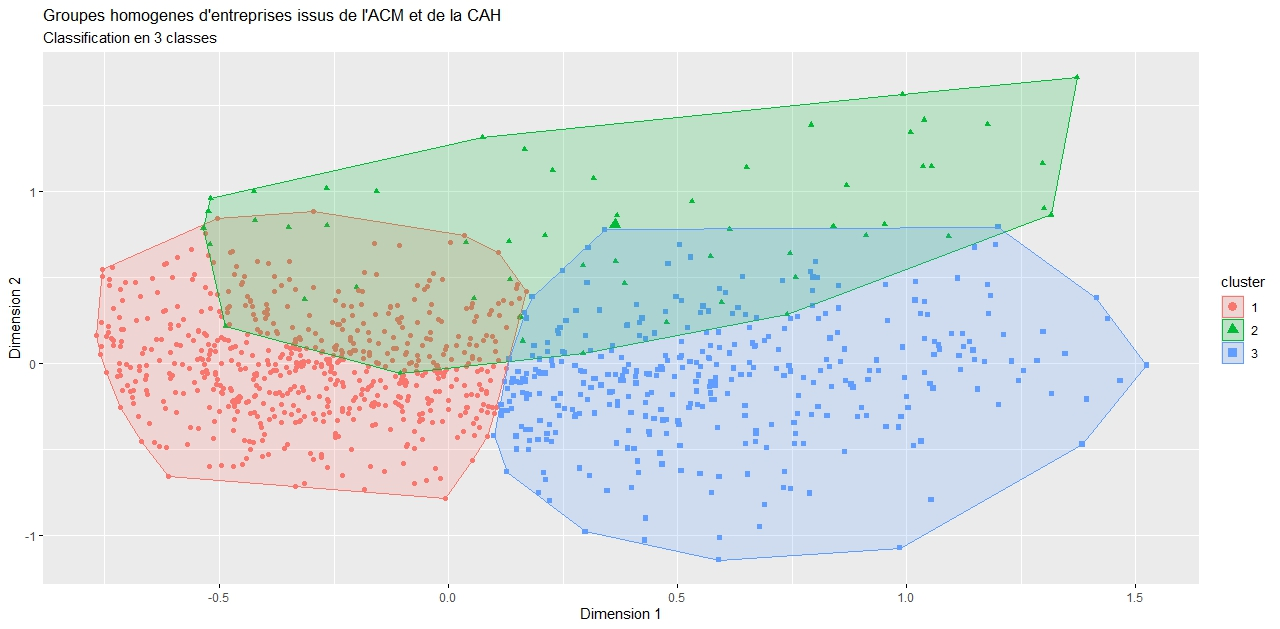
\includegraphics[width=0.68\textwidth]{CAH.jpeg}
	\end{center}
	\begin{block}{Validation de la Cohérence des Groupes}
		\begin{itemize}
			\item Les trois classes occupent des \textbf{zones bien distinctes} du plan factoriel.
			\item Excellente homogénéité intra-classe et séparation inter-classes satisfaisante.
			\item Le croisement ACM-CAH permet de segmenter efficacement le tissu économique.
		\end{itemize}
	\end{block}
\end{frame}


% --- DIAPOSITIVE 3 : Profiling des Classes (Tableau) ---
\begin{frame}{Profil Dominant des Trois Classes Obtenues}
	\begin{center}
		\scriptsize
		\renewcommand{\arraystretch}{1.2}
		\begin{tabular}{l|c|c|c}
			\toprule
			\textbf{Caractéristiques} & \textbf{Classe 1 ($63,1\,\%$)} & \textbf{Classe 2 ($4,8\,\%$)} & \textbf{Classe 3 ($32,2\,\%$)} \\
			\textbf{Dominantes} & \textit{753 entreprises} & \textit{57 entreprises} & \textit{384 entreprises} \\
			\midrule
			
			\textbf{Ancienneté} & 5 à 9 ans ($40,2\,\%$) & Plus de 20 ans ($26,4\,\%$) & 5 à 9 ans ($38,8\,\%$) \\
			
			\rowcolor{gray!5}
			\textbf{Secteur} & \textbf{Agri. / Agroalim.} ($81,1\,\%$) & Services Fin. ($24,6\,\%$) & Agri. / Agroalim. ($31,2\,\%$) \\
			
			\textbf{Région} & Centre ($36,3\,\%$) & Centre ($45,5\,\%$) & Centre ($45,6\,\%$) \\
			
			\rowcolor{gray!5}
			\textbf{Taille} & \alert{\textbf{Petite Entr.}} ($52,5\,\%$) & \alert{\textbf{Moyenne Entr.}} ($54,4\,\%$) & \alert{\textbf{Petite Entr.}} ($59,6\,\%$) \\
			
			\bottomrule
		\end{tabular}
	\end{center}
	
	\begin{block}{Résumé}
		\begin{itemize}
			\tiny
			\item \textbf{Classe 1 (Cœur de cible) :} Majorité d'agro-pME installées en phase de consolidation (5-9 ans).
			\item \textbf{Classe 2 (Grands comptes) :} Entreprises matures, plus grandes, orientées vers le secteur financier.
			\item \textbf{Classe 3 (Profil intermédiaire) :} Petites entreprises du Centre, diversifiées mais à fort ancrage agricole.
		\end{itemize}
	\end{block}

\end{frame}
% -----------------------------------------------------------
%  DIAPO 10 — AFD : vecteurs discriminants
% -----------------------------------------------------------
\begin{frame}{AFD — Vecteurs discriminants (Fisher, 1936)}
    \begin{columns}[T]
        \begin{column}{0.48\textwidth}
            \begin{block}{Décomposition de la variance}
                \[
                    \mathbf{T} = \underbrace{\mathbf{W}}_{\text{intra}}
                               + \underbrace{\mathbf{B}}_{\text{inter}}
                \]
                Critère de Fisher~:
                \[
                    \mathbf{a}^* =
                    \underset{\mathbf{a}}{\arg\max}\;
                    \frac{\mathbf{a}^{\top}\mathbf{B}\,\mathbf{a}}
                         {\mathbf{a}^{\top}\mathbf{W}\,\mathbf{a}}
                \]
            \end{block}
        \end{column}
        \begin{column}{0.48\textwidth}
            \begin{block}{Problème aux valeurs propres}
                \[
                    \mathbf{W}^{-1}\mathbf{B}\,\mathbf{a}_s
                    = \lambda_s\,\mathbf{a}_s
                \]
                Part de discrimination de l'axe $s$~:
                \[
                    \tau_s =
                    \frac{\lambda_s}{\sum_{s'} \lambda_{s'}}
                \]
                \vspace{2pt}
                \textbf{Résultat obtenu~:}\\
                LD1 : 58,6\,\% \quad LD2 : 41,4\,\%\\
                $\Rightarrow$ \textbf{100\,\% en 2 axes}
            \end{block}
        \end{column}
    \end{columns}
\end{frame}

% -----------------------------------------------------------
%  DIAPO 11 — AFD : règle de classification bayésienne
% -----------------------------------------------------------
\begin{frame}{AFD — Règle de classification bayésienne}
    \begin{block}{Score discriminant de Bayes}
        \[
            \delta_c(\mathbf{x}_i)
            = \mathbf{x}_i^{\top}\boldsymbol{\Sigma}^{-1}\boldsymbol{\mu}_c
            - \tfrac{1}{2}\,\boldsymbol{\mu}_c^{\top}
              \boldsymbol{\Sigma}^{-1}\boldsymbol{\mu}_c
            + \log(\pi_c)
        \]
    \end{block}
    \vspace{4pt}
    \begin{columns}[T]
        \begin{column}{0.48\textwidth}
            \begin{block}{Règle de décision}
                \[
                    \hat{c}(\mathbf{x}_i)
                    = \underset{c}{\arg\max}\;
                      \delta_c(\mathbf{x}_i)
                \]
                \small Implémenté via \texttt{MASS::lda()} en R.\\
                La décision repose sur les \textbf{probabilités
                a posteriori} $P(\mathcal{C}_c \mid \mathbf{x}_i)$.
            \end{block}
        \end{column}
        \begin{column}{0.48\textwidth}
            \begin{exampleblock}{Interprétation géométrique}
                Équivalent à affecter l'individu à la classe dont
                le centroïde est le plus proche au sens de la
                \textbf{distance de Mahalanobis} corrigée des
                probabilités a priori $\pi_c = n_c / n$.
            \end{exampleblock}
        \end{column}
    \end{columns}
\end{frame}
% --- DIAPOSITIVE 1 : Projection et Séparation des Classes ---
\begin{frame}{AFD : Validation de la Séparation des Classes}
	\begin{columns}[c]
		\begin{column}{0.55\textwidth}
			\begin{figure}
				\centering
				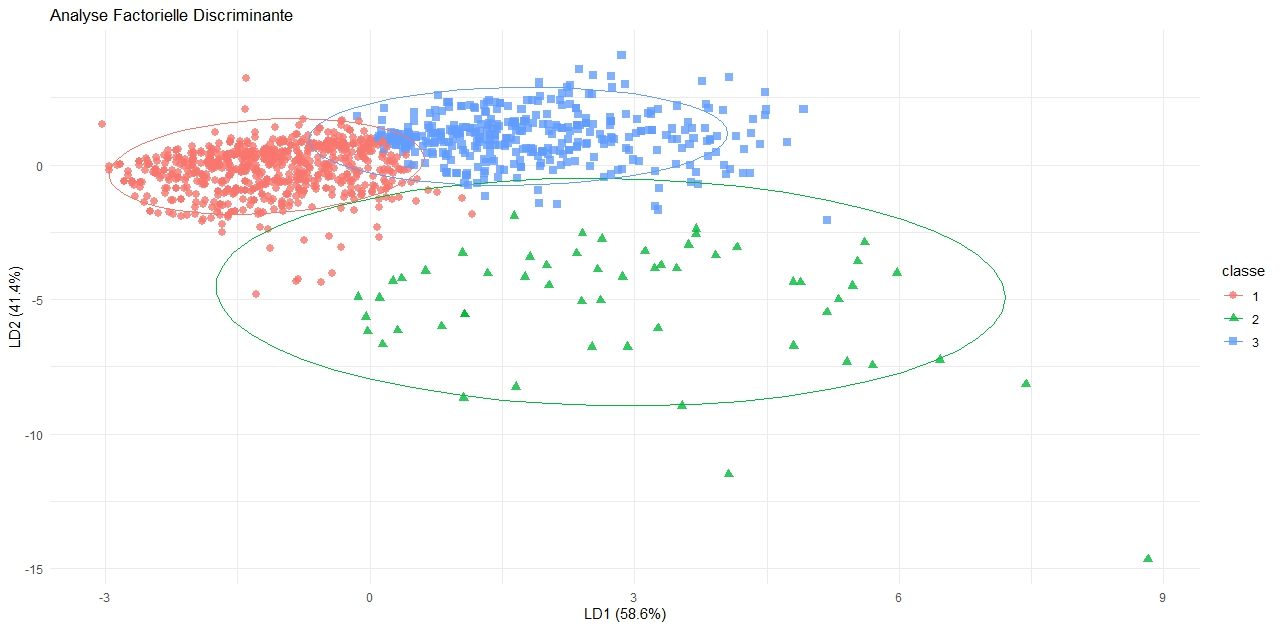
\includegraphics[width=\textwidth]{AFDProjectionDesObservations.jpeg}
				\caption{Projection des observations sur les axes discriminants}
			\end{figure}
		\end{column}
		
		\begin{column}{0.42\textwidth}
			\textbf{Pouvoir discriminant total :}
			\begin{itemize}
				\item \alert{\textbf{100\,\% de l'inertie}} captés par le premier plan factoriel.
				\item \textbf{LD1 :} 58,6\,\% de séparation.
				\item \textbf{LD2 :} 41,4\,\% de séparation.
			\end{itemize}
			\vfill
			\textbf{Pertinence statistique :}
			\begin{itemize}
				\item Séparation globale optimale des trois classes.
				\item Ellipses de confiance à 95\,\% bien distinctes.
				\item \textit{Note :} Léger chevauchement mineur entre la Classe 1 et la Classe 3.
			\end{itemize}
		\end{column}
	\end{columns}
\end{frame}


% --- DIAPOSITIVE 2 : Équations et Rôle des fonctions discriminantes ---
\begin{frame}{Coefficients des Variables sur les Axes LD1 et LD2}
	\begin{columns}[c]
		\begin{column}{0.48\textwidth}
			\begin{center}
				\footnotesize
				\renewcommand{\arraystretch}{1.2}
				\begin{tabular}{l|rr}
					\toprule
					\textbf{Variables (ACM)} & \textbf{LD1} & \textbf{LD2} \\
					\midrule
					\textbf{Dim1} & \cellcolor{red!15}\textbf{3,4117} & 0,8420 \\
					\rowcolor{gray!5}
					\textbf{Dim2} & 0,5020 & \cellcolor{blue!15}\textbf{$-$2,8215} \\
					\textbf{Dim3} & 1,0018 & \cellcolor{blue!15}\textbf{$-$2,3454} \\
					\rowcolor{gray!5}
					\textbf{Dim4} & 0,7551 & \cellcolor{blue!15}\textbf{$-$2,1043} \\
					\textbf{Dim5} & $-$0,5523 & 1,0850 \\
					\bottomrule
				\end{tabular}
			\end{center}
		\end{column}
		
		\begin{column}{0.5\textwidth}
			\begin{block}{Fonction LD1 : Axe Principal}
				\begin{itemize}
					\scriptsize
					\item Largement dominée par \textbf{Dim1} (3,41).
					\item Représente la dimension de discrimination la plus puissante issue des besoins de l'ACM.
				\end{itemize}
			\end{block}
			
			\begin{block}{Fonction LD2 : Axe Secondaire}
				\begin{itemize}
					\scriptsize
					\item Oppose fortement \textbf{Dim2, Dim3 et Dim4} (coefficients négatifs marqués) à Dim1 et Dim5.
					\item Capte une variation orthogonale pour affiner la séparation des groupes restants.
				\end{itemize}
			\end{block}
		\end{column}
	\end{columns}
\end{frame}


% --- DIAPOSITIVE 3 : Indicateurs de Performance ---
\begin{frame}{Indicateurs de Performance du Modèle Discriminant}
	\begin{center}
		\small
		\renewcommand{\arraystretch}{1.2}
		\begin{tabular}{l|c|l}
			\toprule
			\textbf{Indicateur} & \textbf{Valeur} & \textbf{Interprétation de l'expert} \\
			\midrule
			\textbf{Accuracy (Précision)} & \textbf{97,24\,\%} & Classification globale excellente [96,1\% -- 98,1\%] \\
			\rowcolor{gray!5}
			\textbf{Kappa de Cohen} & \textbf{0,9435} & Accord quasi-parfait (corrige l'effet du hasard) \\
			\textbf{Accuracy Null} & 63,07\,\% & Performance d'un classifieur naïf \\
			\rowcolor{gray!5}
			\textbf{Gain de performance} & \alert{\textbf{+34,17\,\%}} & Apport réel et massif du modèle discriminant \\
			\bottomrule
		\end{tabular}
	\end{center}
	
	\vfill
	
	\begin{block}{Significativité Statistique ($p < 0,05$)}
		\begin{itemize}
			\small
			\item \textbf{p-valeur globale :} $5,16 \times 10^{-183} \rightarrow$ Modèle infiniment supérieur à un choix aléatoire.
			\item \textbf{Test de McNemar :} ($p = 8,50 \times 10^{-7}$) Erreurs du modèle non uniformément réparties entre les classes.
		\end{itemize}
	\end{block}
\end{frame}
% ============================================================

% ============================================================
\section{Conclusion}
% ============================================================

% -----------------------------------------------------------
%  DIAPO 18 — CONCLUSION
% -----------------------------------------------------------
\begin{frame}{Conclusion}
    \begin{block}{Ce que ce travail apporte}
        Ce mémoire propose une démarche intégrée, de la
        \textbf{collecte des données terrain} à la
        \textbf{conception d'un outil numérique opérationnel},
        pour répondre à un besoin institutionnel réel du MINEPAT~:
        mieux connaître les entreprises camerounaises pour
        mieux les soutenir.
    \end{block}
    \vspace{10pt}
    \begin{columns}[T]
        \begin{column}{0.48\textwidth}
            \begin{exampleblock}{Contributions méthodologiques}
                Pipeline ACM $\to$ CAH $\to$ AFD appliqué à des
                données qualitatives d'enquête à grande échelle.
                Modèle de classification atteignant
                \textbf{97,24\,\%} de précision.
            \end{exampleblock}
        \end{column}
        \begin{column}{0.48\textwidth}
            \begin{exampleblock}{Contributions opérationnelles}
                Plateforme gouvernementale de cartographie
                et de mise en relation, directement utilisable
                par les agents de la DAPE-MINEPAT.
            \end{exampleblock}
        \end{column}
    \end{columns}
    \vspace{12pt}
    \centering
    \Large\textcolor{primary}{\textbf{Merci de votre attention}}\\[6pt]
    \normalsize\textcolor{darkgray}{Questions et remarques bienvenues}
\end{frame}

\end{document}
